\documentclass[9pt,xcolor=dvipsnames,t]{beamer}
\usetheme{Warsaw}
\usefonttheme[]{serif}
\setbeamertemplate{caption}[numbered]
\setbeamertemplate{footline}[frame number]
\usepackage{amsmath,amssymb,bm,color,graphicx,mathtools} 
\usepackage{fancybox}
\usepackage{fontawesome5}
\usepackage{subfigure}
\usepackage{csquotes}
\usepackage{stmaryrd}
\setbeamercovered{transparent}
\usepackage{animate}
\usepackage{multimedia}
%
\newcommand{\average}[1]{\{\!\!\{#1\}\!\!\}}
\newcommand{\jump}[1]{\llbracket#1\rrbracket}
%
\setbeamersize{text margin left=5mm, text margin right=5mm}
\AtBeginSection[]{
\begin{frame}
    \tableofcontents[currentsection]
\end{frame}}
\usepackage{ragged2e}
\apptocmd{\frame}{}{\justifying}{}
%
\DeclareMathAlphabet{\altmathcal}{OMS}{cmsy}{m}{n}
%https://tex.stackexchange.com/questions/391410/calligraphic-symbols-are-too-fancy-with-mathptmx-package
\usepackage{mathptmx}
\usepackage{tgpagella}
%          {mathpazo}
%          {pxfonts}
%https://latex.org/forum/viewtopic.php?t=10067
\usepackage[bbgreekl]{mathbbol}
%
\usepackage{hyperref}
\newcommand{\crefeq}[1]{Eq.~(\hyperref[#1]{\textcolor{blue}{\ref*{#1}}})}
\hypersetup{
    colorlinks=true,
    citecolor=blue,
    linkcolor=.,
    urlcolor=.
}
%
\usepackage[acronym]{glossaries}
\glsdisablehyper
\newacronym{dg}{DG}{Discontinuous Galerkin}
\newacronym{2d}{2D}{two-dimensional}
\newcommand{\transpose}{^{\mathsf{T}}}
%
%https://tex.stackexchange.com/questions/140619/visual-counter-for-latex
\usepackage{enumitem}
\usepackage{refcount}
\usepackage{tikz}
\usetikzlibrary{calc}
\makeatletter
\newcommand\statuslabel[3][]{%
\def\scale{#1}
\ifx\scale\empty\def\scale{1}\fi
\let\no\relax
\let\n\relax
\newcommand\no{#2}
\newcommand\n{#3}
\def\colorbef{blue}
\def\colorat{blue}
\def\coloraft{black!40}
\let\stop\relax
\sbox\z@{\@tempcnta=0\no\relax}\ifdim\wd0>\z@\relax\@latex@warning{Not a number (#2):\no}\def\stop{1}\fi
\sbox\z@{\@tempcnta=0\n\relax}\ifdim\wd0>\z@\relax\@latex@warning{Not a number (#3): \n}\def\stop{1}\fi
\ifx\stop\relax
\ifnum\no>\n\@latex@warning{Wrong parameter order?}\def\stop{1}\fi
\fi
\ifx\stop\relax
\else
\def\no{1}
\def\n{1}
\def\colorat{red}
\def\stop{??}
\fi
\begin{tikzpicture}[scale=0.1*\scale, baseline={(0,-0.095cm)}]
\def\radiusout{2cm}
\def\radiusin{1.3cm}
\ifnum\n=1
\def\margin{0}
\else
\def\margin{25/\n}
\fi
\foreach\s in {1,...,\n}{
\node[circle, scale=\scale] at (0,0) {\tiny\stop};
\fill[\ifnum\s>\no\coloraft\relax\else\ifnum\s<\no\colorbef\else\colorat\fi\fi]({90-360/\n * (\s - 1)-\margin}:\radiusout) arc ({90-360/\n * (\s - 1)-\margin}:{90-360/\n * (\s)+\margin}:\radiusout) -- ({90-360/\n * (\s)+\margin}:\radiusin) arc ({90-360/\n * (\s)+\margin}:{90-360/\n * (\s - 1)-\margin}:\radiusin);}
\end{tikzpicture}}
\makeatother
\makeatletter
\newcounter{myenum}
\newenvironment{myenum}{\stepcounter{myenum}
\edef\nref{\getrefnumber{myenum@\arabic{myenum}}}
\edef\nref{\expandafter\@firstofone\nref}
\begin{enumerate}[label=\protect\statuslabel{\arabic*}{\nref},ref=\arabic*]}{\label{myenum@\arabic{myenum}}
\end{enumerate}}
\makeatother
%--------------------------------------------------------------
%--------------------------------------------------------------
%--------------------------------------------------------------
% Title page
\title[R\'{e}union DRP/R3C]{R\'{e}union d'unit\'{e} (DRP/R3C)}
\author{Filipe Forte Tenreiro \texorpdfstring{\\}{} [0.50em] \footnotesize{\textit{Sous la supervision} de M. Kazolea\texorpdfstring{\textsuperscript{a}}{} et A. G. Filippini\texorpdfstring{\textsuperscript{b}}{}} \texorpdfstring{\\}{} [0.25em] \texorpdfstring{\textsuperscript{a}}{}\tiny{INRIA Center of the University of Bordeaux - CARDAMOM team - 200 av. de la Vieille Tour, 33405 Talence, France} \texorpdfstring{\\}{} [0.25em] \texorpdfstring{\textsuperscript{b}}{}\tiny{BRGM, French Geological Survey - Coastal Risks and Climate Change team (DRP/R3C) - 3 av. Guillemin, 45100 Orl{\'{e}}ans, France}}
\institute[EDMI, Universit\'{e} de Bordeaux]{
\footnotesize{\'{E}cole Doctorale de Math\'{e}matiques et Informatique (EDMI) \\ Universit\'{e} de Bordeaux}}
\date[Nov 20, 2025]{\footnotesize{Novembre 20, 2025}}
% BEGIN
\begin{document}
\maketitle
% Table of contents
\begin{frame}
\tableofcontents
\end{frame}
% Introduction
\section{Introduction}
%
\subsection*{Motivation}
\begin{frame}
\end{frame}
%
\subsection*{Shallow water asymptotics}
\begin{frame}
\begin{equation}
\begin{aligned}
\text{Shallow water regime: } & \mu\coloneq\frac{h_{0}^{2}}{\lambda^{2}}\ll 1 \\
\text{Large amplitude regime: } & \epsilon\coloneqq\frac{a}{h_{0}}=\altmathcal{O}(1)
\end{aligned}
\end{equation}
\end{frame}
%
\subsection*{The \textit{Green-Naghdi} model}
\begin{frame}
Following \cite{pres_1,pres_2}, the \textit{Green-Naghdi} equations can be written in terms of $\displaystyle{\mathbf{w}=(\eta,q)}$ as follows:
\begin{equation}
\begin{aligned}
\partial_{t}\eta+\partial_{x}q & = 0 \\
(1+\alpha\mathbf{T}[H,b])\left(\partial_{t}q+\partial_{x}(uq)+\frac{\alpha-1}{\alpha}\mathrm{g}H\partial_{x}\eta\right)+\frac{1}{\alpha}\mathrm{g}H\partial_{x}\eta+H\altmathcal{Q}_{1}[H,b](u) & = 0
\end{aligned}
\end{equation}
\end{frame}
\begin{frame}
Following \cite{pres_1,pres_2}, \textit{Green-Naghdi} equations can be written in terms of $\displaystyle{\mathbf{w}=(\eta,q)}$ as follows:
\begin{equation}
\begin{aligned}
\partial_{t}\eta+\partial_{x}q & = 0 \\
\partial_{t}(hu)+\partial_{x}(hu^{2})+\mathrm{g}H\partial_{x}\eta+\textcolor{red}{\mathfrak{d}} & = 0 \\
(1+\alpha\mathbf{T}[H,b])\left(\textcolor{red}{\mathfrak{d}}+\frac{1}{\alpha}\mathrm{g}H\partial_{x}\eta\right) & = \frac{1}{\alpha}\mathrm{g}H\partial_{x}\eta+H\altmathcal{Q}_{1}[H,b](u)
\end{aligned}
\label{Equation: GN (1)}
\end{equation}
\pause
where the linear operator $\displaystyle{\mathbf{T}[H,b](\cdot)}$ and the quadratic form $\displaystyle{\altmathcal{Q}_{1}[H,b](\cdot)}$ are defined for all smooth enough scalar-valued functions $\displaystyle{w}$ by
\begin{equation}
\begin{aligned}
\mathbf{T}[H,b](w) & \coloneqq H\altmathcal{T}[H,b]\left(\frac{w}{H}\right) \\ \altmathcal{Q}_{1}[H,b](w) & \coloneqq -2\altmathcal{R}_{1}[H,b]((\partial_{x}w)^{2})+\altmathcal{R}_{2}[H,b]((w\partial_{x})^{2}b).
\end{aligned}
\end{equation}
\end{frame}
\begin{frame}
As shown in the aforementioned references, \crefeq{Equation: GN (1)} can be recast as
\begin{equation}
\begin{aligned}
\partial_{t}\mathbf{w}+\partial_{x}\mathbb{f}(\mathbf{w},b)+\textcolor{red}{\mathbb{d}(\mathbf{w},b)} & = \mathbb{b}(\mathbf{w},b) & \\ (1+\alpha\mathbf{T}[H, b])\left(\textcolor{red}{\mathfrak{d}}+\frac{1}{\alpha}\mathrm{g}H\partial_{x}\eta\right) & = \frac{1}{\alpha}\mathrm{g}H\partial_{x}\eta+H\altmathcal{Q}_{1}[H, b](u)
\end{aligned}
\end{equation}
\pause
where
\begin{equation}
    \underbrace{\mathbb{f}(\mathbf{w},b)\coloneqq
    \begin{pmatrix}
    q \\ \mathfrak{f}(\mathbf{w},b)\end{pmatrix}}_{\text{\enquote{Shallow-water} flux}},\quad\underbrace{\mathbb{b}(\mathbf{w},b)\coloneqq\begin{pmatrix}0 \\ -\mathrm{g}H\partial_{x}b\end{pmatrix}}_{\text{Source term}},\quad\textcolor{red}{\underbrace{\mathbb{d}(\mathbf{w},b)\coloneqq\begin{pmatrix}0 \\ \mathfrak{d}
    \end{pmatrix}}_{\text{Dispersive correction}}}
\end{equation}
and the nonlinear \textit{pre-balanced} flux is defined as (see \cite{pres_3}):
\begin{equation}
    \mathfrak{f}(\mathbf{w},b)\coloneqq hu^{2}+\frac{1}{2}\mathrm{g}(\eta^{2}-2\eta b).
\end{equation}
\end{frame}
% Discrete formulation
\section{Discrete formulation}
%
\subsection*{High-order Finite Volume (FV) methods}
\begin{frame}[c]
\begin{figure}[!htb]
    \hspace*{\fill}
    \subfigure[Linear ($\displaystyle{\mathbb{P}^{1}}$).]
    {\includegraphics[height=0.30\linewidth]{Figures/DG/Polynomial reconstruction (FV)/PR (1.1).pdf}}
    \hspace{0.1cm}
    \subfigure[Quadratic ($\displaystyle{\mathbb{P}^{2}}$).]
    {\includegraphics[height=0.30\linewidth]{Figures/DG/Polynomial reconstruction (FV)/PR (1.2).pdf}}
    \hspace{0.1cm}
    \subfigure[Cubic ($\displaystyle{\mathbb{P}^{3}}$).]
    {\includegraphics[height=0.30\linewidth]{Figures/DG/Polynomial reconstruction (FV)/PR (1.3).pdf}}
    \hspace*{\fill}
    \vspace{-0.5\baselineskip}
    \caption{Polynomial reconstructions about the \textit{face}.}
\end{figure}
\end{frame}
\begin{frame}[c]
\begin{figure}[!htb]
    \hspace*{\fill}
    \subfigure[$\displaystyle{\mathbb{P}^{1}}$: $\displaystyle{3}$ \textit{monomials}.]
    {\includegraphics[height=0.300\linewidth]{Figures/DG/Discretisation stencil (FV)/DS (1.1).pdf}}
    \hspace{0.1cm}
    \subfigure[$\displaystyle{\mathbb{P}^{2}}$: $\displaystyle{6}$ \textit{monomials}.]
    {\includegraphics[height=0.300\linewidth]{Figures/DG/Discretisation stencil (FV)/DS (1.2).pdf}}
    \hspace{0.1cm}
    \subfigure[$\displaystyle{\mathbb{P}^{n}}$: $\displaystyle{\binom{n+2}{n}}$ \textit{monomials}.]
    {\includegraphics[height=0.300\linewidth]{Figures/DG/Discretisation stencil (FV)/DS (1.3).pdf}}
    \hspace*{\fill}
    \vspace{-0.5\baselineskip}
    \caption{Discretisation stencils for a \textit{least-squares} reconstruction on a cartesian mesh.}
\end{figure}
\end{frame}
%
\subsection*{High-order Discontinuous Galerkin (DG) methods}
\begin{frame}[c]
\begin{figure}[!htb]
    \hspace*{\fill}
    \subfigure[Finite volume.]
    {\includegraphics[height=0.450\linewidth]{Figures/DG/Discretisation stencil (FV)/DS (2.1).pdf}}
    \hspace{0.1cm}
    \subfigure[\gls{dg}.]
    {\includegraphics[height=0.450\linewidth]{Figures/DG/Discretisation stencil (FV)/DS (2.2).pdf}}
    \hspace*{\fill}
    \vspace{-0.5\baselineskip}
    \caption{Discretisation stencils for \textit{arbitrarily} higher-order reconstructions about the \textit{face} in red.}
\end{figure}
\end{frame}
\begin{frame}[c]
\begin{figure}[!htb]
    {\includegraphics[height=0.195\linewidth]{Figures/DG/Cell/CELL_PAMPA_VERT_LOCAL.pdf}}
    \vspace{-0.5\baselineskip}
    \caption{\textit{Local} partitions.}
\end{figure}
\vspace{-0.5\baselineskip}
\begin{figure}[!htb]
    \hspace*{\fill}
    \subfigure[Partition $\displaystyle{1}$.]
    {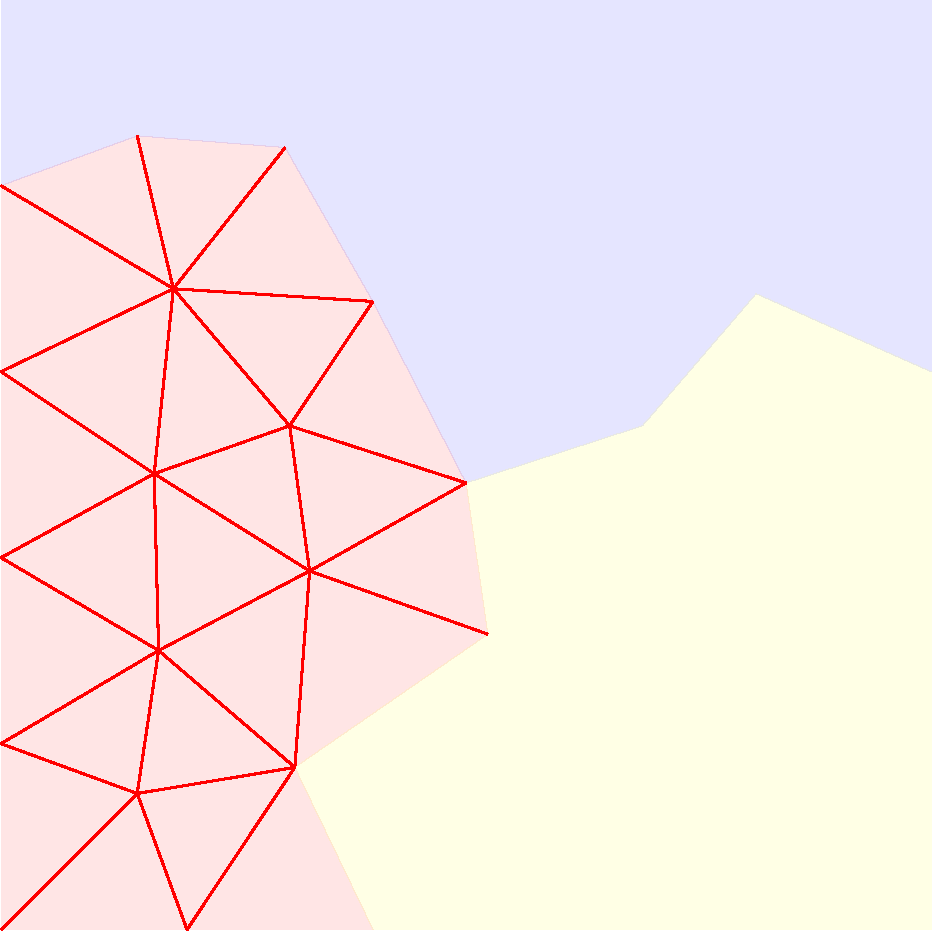
\includegraphics[height=0.195\linewidth]{Figures/DG/Face/FACE_PAMPA_VERT_LOCAL_AND_NOT_FRONTIER_0.pdf}}
    \hspace{0.1cm}
    \subfigure[Partition $\displaystyle{2}$.]
    {\includegraphics[height=0.195\linewidth]{Figures/DG/Face/FACE_PAMPA_VERT_LOCAL_AND_NOT_FRONTIER_1.pdf}}
    \hspace{0.1cm}
    \subfigure[Partition $\displaystyle{3}$.]
    {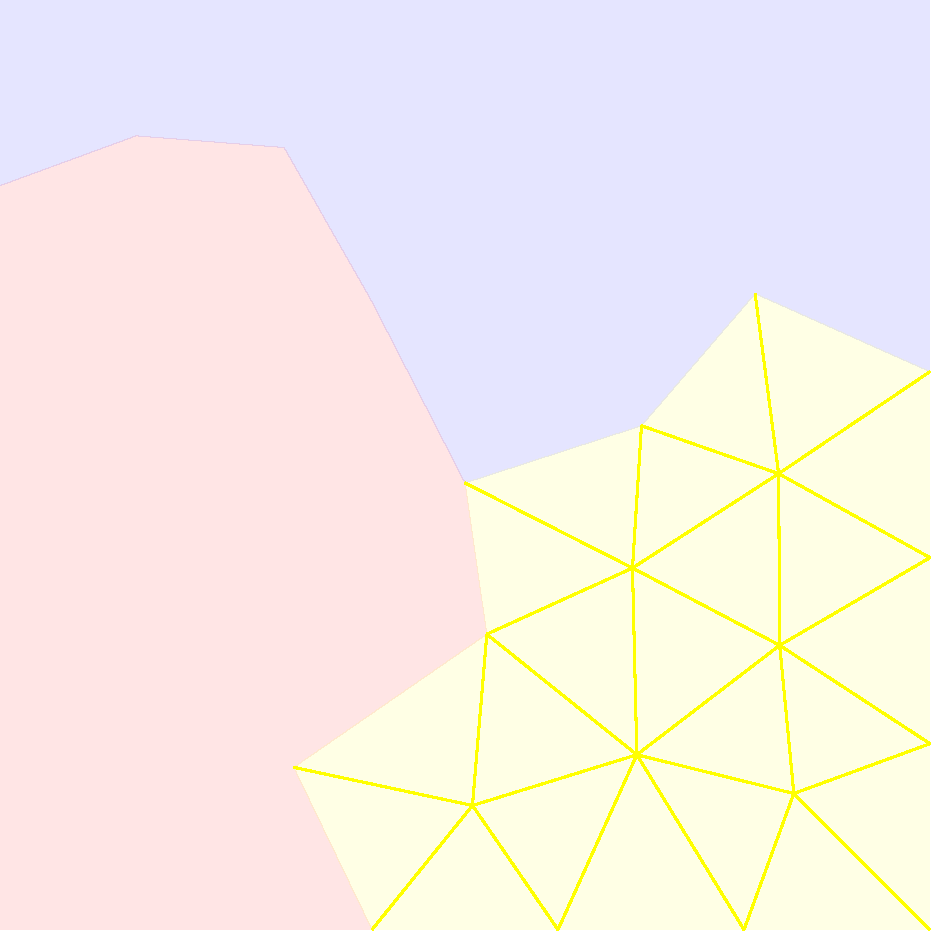
\includegraphics[height=0.195\linewidth]{Figures/DG/Face/FACE_PAMPA_VERT_LOCAL_AND_NOT_FRONTIER_2.pdf}}
    \hspace*{\fill}
    \vspace{-0.5\baselineskip}
    \caption{\textit{Local and non-frontier} partitions.}
\end{figure}
\end{frame}
\begin{frame}[c]
\begin{figure}[!htb]
    \hspace*{\fill}
    \subfigure[Partition $\displaystyle{1}$.]
    {\includegraphics[height=0.195\linewidth]{Figures/DG/Cell/CELL_PAMPA_VERT_OVERLAP_0.pdf}}
    \hspace{0.1cm}
    \subfigure[Partition $\displaystyle{2}$.]
    {\includegraphics[height=0.195\linewidth]{Figures/DG/Cell/CELL_PAMPA_VERT_OVERLAP_1.pdf}}
    \hspace{0.1cm}
    \subfigure[Partition $\displaystyle{3}$.]
    {\includegraphics[height=0.195\linewidth]{Figures/DG/Cell/CELL_PAMPA_VERT_OVERLAP_2.pdf}}
    \hspace*{\fill}
    \vspace{-0.5\baselineskip}
    \caption{\textit{Overlapping} partitions.}
\end{figure}
\vspace{-0.5\baselineskip}
\begin{figure}[!htb]
    \hspace*{\fill}
    \subfigure[Partition $\displaystyle{1}$.]
    {\includegraphics[height=0.195\linewidth]{Figures/DG/Face/FACE_PAMPA_VERT_FRONTIER_0.pdf}}
    \hspace{0.1cm}
    \subfigure[Partition $\displaystyle{2}$.]
    {\includegraphics[height=0.195\linewidth]{Figures/DG/Face/FACE_PAMPA_VERT_FRONTIER_1.pdf}}
    \hspace{0.1cm}
    \subfigure[Partition $\displaystyle{3}$.]
    {\includegraphics[height=0.195\linewidth]{Figures/DG/Face/FACE_PAMPA_VERT_FRONTIER_2.pdf}}
    \hspace*{\fill}
    \vspace{-0.5\baselineskip}
    \caption{\textit{Frontier} partitions.}
\end{figure}
\end{frame}
%
\subsection*{SIPG bilinear form}
\begin{frame}
In this section, we derive \gls{dg} approximations of the model discussed above.
\pause

$\displaystyle{\vphantom{0}}$

For further use, we consider the following bilinear form $\displaystyle{a_{h}(\kappa;\cdot,\cdot)}$ on $\displaystyle{\mathbb{P}^{k}(\altmathcal{T}_{h})\times\mathbb{P}^{k}(\altmathcal{T}_{h})}$:
\begin{equation}
\begin{aligned}
& a_{h}(\kappa;v_{h},w_{h})\coloneqq\sum_{T\in\altmathcal{T}_{h}}\left(\kappa\partial_{x}\nu_{h},\partial_{x}w_{h}\right)_{T}\ldots \\ & -\sum_{F\in\altmathcal{F}_{h}}\Bigg(\Big(\jump{v_{h}},\average{\kappa\partial_{x}^{h}w_{h}}_{\omega}\Big)_{F}-\theta\underbrace{\Big(\average{\kappa\partial_{x}^{h}v_{h}},\jump{w_{h}}_{\omega}\Big)_{F}\vphantom{\left(\frac{\eta_{\kappa,F}}{h_{F}}\right)_{F}}}_{\text{symmetrisation term}}-\underbrace{\left(\frac{\eta_{\kappa,F}}{h_{F}}\jump{v_{h}},\jump{w_{h}}\right)_{F}}_{\text{penalty term}}\Bigg)
\end{aligned}
\label{Equation:Bilinear (1)}
\end{equation}
where $\displaystyle{\theta = -1}$ (SIPG) and $\displaystyle{\eta_{\kappa,F}\geq 0}$ denotes a user-defined parameter sufficiently large to ensure coercivity.

For further reference, see \cite{pres_4}.
\end{frame}
%
\subsection*{Discrete gradient and Laplace operators}
\begin{frame}
To discretise the \textbf{linear} and \textbf{nonlinear} operators in our model, we define the following \textit{global lifting} of the jumps $\displaystyle{v_{h}\in\mathbb{P}^{k}(\altmathcal{T}_{h})}$ (\textit{trial function}):
\begin{equation}
\altmathcal{R}_{h}^{k}(\jump{v_{h}})\coloneqq\sum_{F\in\altmathcal{F}_{h}}r_{F}^{k}(\jump{v_{h}}).
\end{equation}
\pause

Following \cite{pres_5}, we define the discrete gradient operator $\displaystyle{\altmathcal{G}_{h}^{k}\forall v_{h}\in\mathbb{P}^{k}(\altmathcal{T}_{h})}$,
\begin{equation}
\altmathcal{G}_{h}^{k}(v_{h})\coloneqq\partial_{x}^{h}v_{h}-\altmathcal{R}_{h}^{k}(\jump{v_{h}}).
\end{equation}
\pause

Similarly, we introduce the discrete Laplace operator $\displaystyle{\altmathcal{L}_{h}^{k}}$ such that, for all $\displaystyle{v_{h}\in\mathbb{P}^{k}(\altmathcal{T}_{h})}$, $\displaystyle{\altmathcal{L}_{h}^{k}(v_{h})}$ solves
\begin{equation}
-(\altmathcal{L}_{h}^{k}(v_{h}),\psi_{h})_{\Omega}=a_{h}(1;v_{h},\psi_{h}),\quad\forall\psi_{h}\in\mathbb{P}^{k}(\altmathcal{T}_{h})
\end{equation}
where we have set $\displaystyle{\eta_{\kappa,F} = 0}$.
\end{frame}
%
\subsection*{The discrete problem}
\begin{frame}
Provided that the exact solution is \textit{sufficiently} regular, the \textit{Green-Naghdi} model can be rewritten as
\begin{subequations}
\begin{align}
    \partial_{t}\mathbf{w}+\partial_{x}\mathbb{f}(\mathbf{w},b)+\textcolor{red}{\mathbb{d}(\mathbf{w},b)} & = \mathbb{b}(\mathbf{w},b) \\
    H\textcolor{blue}{\mathfrak{p}} & = \textcolor{red}{\mathfrak{d}}+\frac{1}{\alpha}\mathrm{g}H\partial_{x}\eta \label{Equation: GN (4.2)} \\ 
    \partial_{x}\left(-\nu[H]\partial_{x}\textcolor{blue}{\mathfrak{p}}\right)+\beta[H,b]\textcolor{blue}{\mathfrak{p}} & = \frac{1}{\alpha}\mathrm{g}H\partial_{x}\eta+\altmathcal{Q}_{1}[H,b](u)
\end{align}
\end{subequations}
where \crefeq{Equation: GN (4.2)} has to be interpreted as the definition of the auxiliary variable $\displaystyle{\mathfrak{p}}$ and
\begin{equation}
    \nu[H] = \frac{1}{3}H^{3},\quad\beta[H,b] = H+\frac{1}{2}\partial{x}(H^{2}\partial_{x}b)+H(\partial_{x}b)^{2}.
\end{equation}
\pause

\vfill
\footnotesize{\underline{Note:} In a \gls{2d} setting, the $\displaystyle{\mathbf{T}[H,b](\mathbf{w})}$ operator can be rewritten as
\begin{equation}
    \mathbf{T}[H,b](\mathbf{w}) = H\boldsymbol{\nabla}\left(\nu[H]\boldsymbol{\nabla}\cdot\left(\frac{\mathbf{w}}{H}\right)\right)+\beta[H,b]\left(\frac{\mathbf{w}}{H}\right).
\end{equation}
Since the bilinear form $\displaystyle{a_{h}(\kappa;v_{h},w_{h})}$ in \crefeq{Equation:Bilinear (1)} is written in divergence form, it is \textbf{not} a good idea to develop the divergence of the first term of this operator. Instead, it is more practical to solve \crefeq{Equation: GN (3.3)} for $\displaystyle{\mathfrak{p}}$ and then retrieve $\displaystyle{\mathfrak{d}}$ (dispersive correction).}
\end{frame}
\begin{frame}
The semi-discrete \gls{dg} approximation of \crefeq{Equation: GN (1)} now reads: find $\displaystyle{(\eta_{h},u_{h},\textcolor{blue}{\mathfrak{p}_{h}})\in(\mathbb{P}^{k}(\altmathcal{T}_{h}))^{3}}$ such that, for all $\displaystyle{(\psi_{h},\phi_{h},\varphi_{h})\in(\mathbb{P}^{k}(\altmathcal{T}_{h}))^{3}}$,
\begin{subequations}
\begin{align}
(\partial_{t}\mathbf{w}_{h},\varphi_{h})_{\Omega}+\left(\altmathcal{A}_{h}(\mathbf{w}_{h}),\varphi_{h}\right)_{\Omega} & = 0 \label{Equation: GN (3.1)} \\ 
(H_{h}\mathfrak{p}_{h},\phi_{h})_{\Omega} & = (\textcolor{red}{\mathfrak{d}_{h}},\phi_{h})_{\Omega}+\left(\frac{1}{\alpha}\mathrm{g}H_{h}\altmathcal{G}_{h}^{k}(\eta_{h}),\phi_{h}\right)_{\Omega} \label{Equation: GN (3.2)} \\ 
a_{h}(\nu[H_{h}];\textcolor{blue}{\mathfrak{p}_{h}},\psi_{h})+(\beta_{h}[H_{h},b_{h}]\textcolor{blue}{\mathfrak{p}_{h}},\psi_{h})_{\Omega} & = (\mathbb{Q}_{h}^{(1)}[H_{h},b_{h}](\eta_{h},u_{h}),\psi_{h})_{\Omega}. \label{Equation: GN (3.3)}
\end{align}
\end{subequations}

$\displaystyle{\vphantom{0}}$

\begin{myenum}
    \item Solve the linear system in \crefeq{Equation: GN (3.3)} for $\displaystyle{\textcolor{blue}{\mathfrak{p}_{h}}}$.
    \item Compute the dispersive correction $\displaystyle{\textcolor{red}{\mathfrak{d}_{h}}}$ in \crefeq{Equation: GN (3.2)} and add it as a \textit{source term} to the nonlinear operator $\displaystyle{\altmathcal{A}_{h}}$ in \crefeq{Equation: GN (3.1)}.
    \item Evolve $\displaystyle{\mathbf{w}(\eta_{h},u_{h})}$ \textit{in time}.
\end{myenum}
\end{frame}
\begin{frame}
$\displaystyle{\textcolor{blue}{(\mathbf{1})}}$ The discrete \textbf{nonlinear} operator $\displaystyle{\altmathcal{A}_{h}}$ in \crefeq{Equation: GN (3.1)} is defined by
\begin{equation}
\begin{aligned}
    (\altmathcal{A}_{h} & (\mathbf{w}_{h}),\varphi_{h})_{\Omega} \coloneqq \\ & -\sum_{T\in\altmathcal{T}_{h}}\left(\mathbb{f}(\mathbf{w}_{h},b_{h}),\partial_{x}\varphi_{h}\right)_{T}+\sum_{T\in\altmathcal{T}_{h}}\sum_{F\in\altmathcal{F}_{T}}(\widehat{\mathbb{f}}_{TF},\varphi_{h})_{F}-\left(\mathbb{b}(\mathbf{w}_{h},b_{h}),\varphi_{h}\right)_{\Omega}+\textcolor{red}{\left(\mathbb{d}_{h},\varphi_{h}\right)_{\Omega}}
\end{aligned}
\end{equation}
with discrete \textbf{dispersive correction} $\displaystyle{\textcolor{red}{\mathbb{d}_{h}\coloneqq\begin{bmatrix} 0 \\ \mathfrak{d}_h\end{bmatrix}}\in(\mathbb{P}^{k}(\altmathcal{T}_{h}))^{2}}$.
Here, $\displaystyle{\widehat{\mathbb{f}}_{TF}}$ is a numerical approximation of the normal face fluxes $\displaystyle{\mathbb{f}(\mathbf{w}_{h},b_{h})\cdot n_{TF}}$.

$\displaystyle{\vphantom{0}}$

\pause
$\displaystyle{\textcolor{blue}{(\mathbf{2})}}$ The discrete \textbf{linear} operator $\displaystyle{\beta_{h}[H_{h},b_{h}]}$ in \crefeq{Equation: GN (3.3)} is defined by
\begin{equation}
    \beta_{h}[H_{h},b_{h}]\coloneqq\underbrace{H_{h}+H_{h}\altmathcal{G}_{h}^{k}(H_{h})\altmathcal{G}_{h}^{k}(b_{h})+\frac{1}{2}H_{h}^{2}\altmathcal{L}_{h}^{k}(b_{h})+H_{h}\altmathcal{G}_{h}^{k}(b_{h})^{2}}_{\equiv\textcolor{red}{h\left(1+h^{\prime}b^{\prime}+\frac{1}{2}hb^{\prime\prime}+{b^{\prime}}^{2}\right)}}.
\end{equation}
\end{frame}
\begin{frame}
$\displaystyle{\textcolor{blue}{(\mathbf{3})}}$ The discrete \textbf{nonlinear} operator $\displaystyle{\mathbb{Q}_{h}^{(1)}[H_{h},b_{h}]}$ in \crefeq{Equation: GN (3.3)} is defined by
\begin{equation}
\mathbb{Q}_{h}^{(1)}[H_{h},b_{h}](\eta_{h},u_{h})\coloneqq\frac{1}{\alpha}\mathrm{g}H_{h}\altmathcal{G}_{h}^{k}(\eta_{h})+H_{h}\altmathcal{Q}_{1,h}[H_{h},b_{h}](u_{h}),
\end{equation}
where, for any $\displaystyle{w_{h}\in\mathbb{P}^{k}(\altmathcal{T}_{h})}$,
\begin{equation}
\begin{aligned}
    \altmathcal{Q}_{1,h}[H_{h},b_{h}](w_{h}) & \coloneqq \underbrace{2H_{h}\altmathcal{G}_{h}^{k}\left(H_{h}+\frac{b_{h}}{2}\right)\altmathcal{G}_{h}^{k}(w_{h})^{2}}_{\textcolor{red}{\equiv 2h\left(h+\frac{b}{2}\right)^{\prime}{u^{\prime}}^{2}}}+\underbrace{\vphantom{\left(\frac{b_{h}}{2}\right)}\frac{4}{3}H_{h}^{2}\altmathcal{G}_{h}^{k}(w_{h})\altmathcal{L}_{h}^{k}(w_{h})}_{\textcolor{red}{\equiv\vphantom{\left(\frac{b_{h}}{2}\right)}\frac{4}{3}h^{2}u^{\prime}u^{\prime\prime}}} \\ & +\underbrace{H_{h}\altmathcal{L}_{h}^{k}(b_{h})w_{h}\altmathcal{G}_{h}^{k}(w_{h})}_{\textcolor{red}{\equiv hb^{\prime\prime}uu^{\prime}}}+\underbrace{\left(\altmathcal{G}_{h}^{k}(\eta_{h})\altmathcal{L}_{h}^{k}(b_{h})+\frac{H_{h}}{2}\altmathcal{G}_{h}^{k}(\altmathcal{L}_{h}^{k}(b_{h}))\right)w_{h}^{2}}_{\textcolor{red}{\equiv \left(\eta^{\prime}b^{\prime\prime}+\frac{h}{2}b^{\prime\prime\prime}\right)u^{2}}}.
\end{aligned}
\end{equation}
\end{frame}
%
% V&V
\section{Verification and Validation (V\&V)}
% #1
\subsection*{Test 1: Nonlinear shallow water equations}
\begin{frame}
\begin{figure}[!htb]
    \hspace*{\fill}
    \subfigure[Free-surface elevation ($\displaystyle{\eta}$).]
    {\includegraphics[height=0.435\linewidth]{Figures/T1/SW_P1 (z, 0.01s).pdf}}
    \subfigure[Momentum ($\displaystyle{q = hu}$).]
    {\includegraphics[height=0.435\linewidth]{Figures/T1/SW_P1 (q, 0.01s).pdf}}
    \hspace*{\fill}
    \vspace{-0.5\baselineskip}
    \caption{Free-surface elevation ($\displaystyle{\eta}$) and momentum ($\displaystyle{q}$) distribution at $\displaystyle{t^{\prime} = 0.01s}$.}
\end{figure}
\end{frame}
\begin{frame}
\begin{figure}[!htb]
    \hspace*{\fill}
    \subfigure[Free-surface elevation ($\displaystyle{\eta}$).]
    {\includegraphics[height=0.435\linewidth]{Figures/T1/SW (z, 0.01s).pdf}}
    \subfigure[Momentum ($\displaystyle{q = hu}$).]
    {\includegraphics[height=0.435\linewidth]{Figures/T1/SW (q, 0.01s).pdf}}
    \hspace*{\fill}
    \vspace{-0.5\baselineskip}
    \caption{Discretisation error norm ($\displaystyle{\ell_{2}}$-norm) decay for increasingly refined uniform grids.}
\end{figure}
\end{frame}
% #2
\subsection*{Test 2: Solitary wave propagation}
% #3
\subsection*{Test 3: Head-on collision and symmetry boundary conditions}
\begin{frame}[c]
\begin{figure}
\begin{minipage}{0.45\linewidth}
    \animategraphics[width=\linewidth,autoplay,loop]{30}{Figures/T3/Hoc/21/}{1}{150}
    \vspace{-0.5\baselineskip}
    \caption{Head-on collision ($\displaystyle{\epsilon=0.21}$).}
\end{minipage}
\hfill
\begin{minipage}{0.45\linewidth}
    \animategraphics[width=\linewidth,autoplay,loop]{30}{Figures/T3/Wall/21/}{1}{150}
    \vspace{-0.5\baselineskip}
    \caption{Wall ($\displaystyle{\epsilon=0.21}$).}
\end{minipage}
\end{figure}
\end{frame}







\begin{frame}[c]
\begin{figure}
\begin{minipage}{0.45\linewidth}
    \animategraphics[width=\linewidth,autoplay,loop]{30}{Figures/T3/Hoc/96/}{1}{150}
    \vspace{-0.5\baselineskip}
    \caption{Head-on collision ($\displaystyle{\epsilon=0.96}$).}
\end{minipage}
\hfill
\begin{minipage}{0.45\linewidth}
    \animategraphics[width=\linewidth,autoplay,loop]{30}{Figures/T3/Wall/96/}{1}{150}
    \vspace{-0.5\baselineskip}
    \caption{Wall ($\displaystyle{\epsilon=0.96}$).}
\end{minipage}
\end{figure}
\end{frame}
\begin{frame}[c]
\begin{figure}[!htb]
    \hspace*{\fill}
    \subfigure[$\displaystyle{\epsilon = 0.21}$.]
    {\includegraphics[height=0.45\linewidth]{Figures/T3/HocWall1_P3 (0.21).pdf}}
    \subfigure[$\displaystyle{\epsilon = 0.96}$.]
    {\includegraphics[height=0.45\linewidth]{Figures/T3/HocWall1_P3 (0.96).pdf}}
    \hspace*{\fill}
    \vspace{-0.5\baselineskip}
    \caption{Free-surface elevation ($\displaystyle{\zeta^{\prime}}$) distribution at $\displaystyle{t^{\prime} = t_{0, p, f}^{\prime}}$ for waves of $\displaystyle{\epsilon = 0.21}$ and $\displaystyle{0.96}$.}
\end{figure}
\end{frame}
% #4
\subsection*{Test 4: Overtaking collision}
\begin{frame}
\end{frame}
% #5
\subsection*{Test 5: Dispersive dam-break}
\begin{frame}[c]
\begin{figure}
\begin{minipage}{0.45\linewidth}
    \animategraphics[width=\linewidth,autoplay,loop]{30}{Figures/T5/frames/h/}{1}{150}
    \vspace{-0.5\baselineskip}
    \caption{X.}
\end{minipage}
\hfill
\begin{minipage}{0.45\linewidth}
    \animategraphics[width=\linewidth,autoplay,loop]{30}{Figures/T5/frames/u/}{1}{150}
    \vspace{-0.5\baselineskip}
    \caption{X.}
\end{minipage}
\end{figure}
\end{frame}
\begin{frame}
\begin{figure}[!htb]
    \hspace*{\fill}
    \subfigure[Water depth ($\displaystyle{h}$).]
    {\includegraphics[height=0.45\linewidth]{Figures/T5/Ddb_h.pdf}}
    \subfigure[Velocity ($\displaystyle{u}$).]
    {\includegraphics[height=0.45\linewidth]{Figures/T5/Ddb_u.pdf}}
    \hspace*{\fill}
    \vspace{-0.5\baselineskip}
    \caption{Water depth ($\displaystyle{h}$) and velocity ($\displaystyle{u}$) distribution at $\displaystyle{t = 47.434s}$.}
\end{figure}
\end{frame}
% #6
\subsection*{Test 6: Grilli \textit{et al.}}
\begin{frame}
\begin{figure}[!htb]
    \hspace*{\fill}
    \subfigure[Incident waves at gauge $\displaystyle{g_{0}}$.]
    {\includegraphics[height=0.45\linewidth]{Figures/T6/Grilli0 (C3, gn).pdf}}
    \subfigure[Shoaling waves at gauges $\displaystyle{g_{1}-g_{9}}$.]
    {\includegraphics[height=0.45\linewidth]{Figures/T6/Grillik (C3, gn).pdf}}
    \hspace*{\fill}
    \vspace{-0.5\baselineskip}
    \caption{Comparison between experiments ($\displaystyle{\circ}$) and computations (\rule[0.5ex]{1em}{0.5pt}).}
\end{figure}
\end{frame}
% #7
\subsection*{Test 7: Reflection of shoaling waves (M. Walkley)}
\begin{frame}[c]
\begin{figure}[!htb]
    \hspace*{\fill}
    \subfigure[$\displaystyle{t = 0s}$.]
    {\includegraphics[height=0.45\linewidth]{Figures/T7/Ref2 (t0).pdf}}
    \subfigure[$\displaystyle{t = 30s}$.]
    {\includegraphics[height=0.45\linewidth]{Figures/T7/Ref2 (tf).pdf}}
    \hspace*{\fill}
    \vspace{-0.5\baselineskip}
    \caption{Experimental setup for waves of $\displaystyle{\epsilon = 0.07}$ (\textcolor{red}{\rule[0.5ex]{1em}{0.5pt}}) and $\displaystyle{0.12}$ (\textcolor{blue}{\rule[0.5ex]{1em}{0.5pt}}).}
\end{figure}
\end{frame}
\begin{figure}
\begin{minipage}{0.45\linewidth}
    \animategraphics[width=\linewidth,autoplay,loop]{30}{Figures/T7/frames/fig1/}{1}{150}
    \vspace{-0.5\baselineskip}
    \caption{Head-on collision ($\displaystyle{\epsilon=0.96}$).}
\end{minipage}
\hfill
\begin{minipage}{0.45\linewidth}
    \animategraphics[width=\linewidth,autoplay,loop]{30}{Figures/T7/frames/fig2/}{1}{150}
    \vspace{-0.5\baselineskip}
    \caption{Wall ($\displaystyle{\epsilon=0.96}$).}
\end{minipage}
\end{figure}
% Appendix
\section{Appendix}
\begin{frame}
\href{https://github.com/FilipeFT24/PhD-presentation}{\textcolor{blue}{\faLink}}\quad Presentation repository (Github)

\href{https://github.com/FilipeFT24/uhainafil-toy1d}{\textcolor{blue}{\faLink}}\quad Uhaina 1D toy code repository (GitHub)

\href{https://mega.nz/folder/I4Y0GKDA\#1VnqBam5Gidli6l3GdMMng}{\textcolor{blue}{\faLink}}\quad PhD repository (MEGA)

$\displaystyle{\vphantom{0}}$

\scriptsize
\bibliography{ref.bib}
\bibliographystyle{apalike}
\end{frame}
\end{document}